% !TeX spellcheck = en_GB
\graphicspath{ {./diagrams/} }
\chapter{Design Diagrams}\label{chapter:Design Diagrams}

\section{Use-case diagram}

\begin{flushleft}
	The use case diagram illustrates how the user interacts with the operating system. There is a total of three interactions between user and the operating system in this case.
	The first interaction that the user initiates is the boot process.\\ 
	This involves:
\end{flushleft}


\begin{enumerate}

	\item \textbf{Setting up interrupts}
	\begin{flushleft}
		The concept behind interrupts is that when a piece of hardware or software wants to
		interrupt the CPU to do something important, an interrupt is raised. The CPU
		executes a program called the ISR (Interrupt Service Routine) and returns back to
		what is was doing before.
	\end{flushleft}

	\item \textbf{Loading VGA driver}
	\begin{flushleft}
		Using VGA to print text to the screen is quite simple and is achieved by using
		VGA text-mode. The user can directly write to the video memory located at
		address 0xB8000. Each character that is to be printed requires a two-byte
		representation:
		1 byte, called the code-point is used to represent the character in ASCII.
		1 byte, is used to set the background and foreground colors. There are 16
		colors that can be used.
		In VGA text-mode a maximum of 80x25 characters can be printed on the
		screen at a time.
	\end{flushleft}

	\item \textbf{Load keyboard driver}
	\begin{flushleft}
		The keyboard driver uses the PS/2 interface to enable communication between the keyboard and the computer. When a key is pressed 
		on the keyboard, the PIC raises IRQ1. This triggers an ISR which on execution will store the pressed key on a circular buffer.
		The data from the circular buffer is read by primitives from the C standard library such as scanf in stdio. The data from keyboard is
		read from port 0x60 using inline assembly function \textbf{inportb()} defined in io.c file.
	\end{flushleft}

	\item \textbf{Setting up memory}
	\begin{flushleft}
		This involves ensuring that multiboot is working as intended and confirming that the 
		\textbf{multiboot\_info\_t} structure contains the fields neccessary for memory management.
		 Other intermediate datastructures needed for memory management such as the stack and global variables
		are also initialized at this stage.
	\end{flushleft}
\end{enumerate}

\begin{flushleft}
The second interaction involves the user issuing a command to the terminal. \\
The command may require dynamic memory to be allocated. Dynamic memory is
allocated by implementing the malloc C function. The malloc function acts as a
wrapper around the kernels memory manager. 
\end{flushleft}




\begin{figure}[h!]
	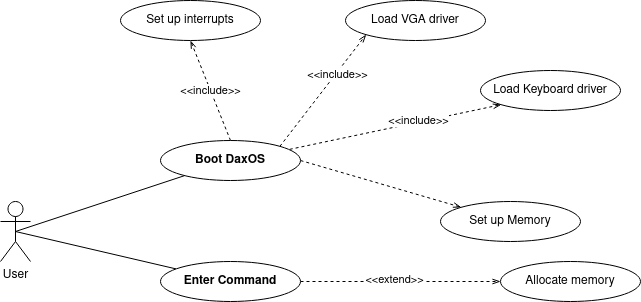
\includegraphics[width=\textwidth,height=\textheight,keepaspectratio]{use-case}
	\caption{Use Case Diagram}
\end{figure}

\pagebreak

\section{Activity Diagram}

\begin{flushleft}
	The activity diagram illustrates the shell scripts that are used to build and compile the kernel.
	
	The most important script here is the \textbf{build.sh} shell script which dives the make
	program to compile our source code. The build script relies further on two other shell
	scripts:
	\begin{enumerate}
		\item \textbf{headers.sh} script
		\begin{flushleft}
			Since in this project a version of C standard library is implemented the compilation of
			kernel is done by instructing the GCC cross-compiler to look for system headers in
			the SYSROOT directory. This script compiles the custom C std-lib into an archive
			named libk.a and places it in the SYSROOT/usr/lib directory.
			Also it copies all the .h header files into SYSROOT/usr/include directory. Now
			compiling the kernel is done by passing the --sysroot=SYSROOT parameter.
		\end{flushleft}
	
		\item \textbf{config.sh} script
		\begin{flushleft}
			This script sets up all the environment variables used by GNU Make.This allows the
			user to easily change the core aspects and tooling used in the projects later. For
			example, we could change the compiler from GCC to CLANG by simply changing
			the environment variable CC to CLANG. Likewise SYSROOT directory can be
			changed by changing a single variable.
			Once these two scripts are executed the build script runs the make-install command
			on each of the folder directory. It copies the output DaxOS.kernel file into the boot
			directory.
		\end{flushleft}
	
	\end{enumerate}

	The \textbf{iso.sh} script builds a bootable .iso image file from our kernel. It first calls the
	previously described build script and then produced an iso file by using the grub-
	mkrescue program. This iso file can be loaded into any emulator to run the operating
	system. The iso files are built into the isodir directory.
	
	\pagebreak
	The \textbf{clean.sh} script removes all the build artifacts from the compilation. Build artifacts
	are files that are produced by the compilation process that can always be
	reproduced by the compiler. Since it can be reproduced it is usually removed to
	maintain a clean project structure.
	
	There are three kinds of build artifacts:
	\begin{enumerate}
		\item  \textbf{Object files} - .o files
		\item  \textbf{Make dependencies} - .d files
		\item  \textbf{Unwanted directories} - sysroot, isodir
	\end{enumerate}

	The clean script works by executing the make clean commands in each of the
	project directories.The make clean commands use the rm bash command to delete
	the build artifacts.
	
	\vspace{1.5 cm}
	
	The last script is the \textbf{create-bootable-usb.sh} script. This script
	creates a bootable USB of the operating system. It needs sudo permission because it accesses the
	UNIX block file of the USB device. This of the form /dev/sda or something similar. 
	This script formats the USB device and copies the kernel along with the GRUB bootloader into the USB device. 
	Therefore there is a chance that the data in the USB device can be destroyed if the user is not careful.
	To prevent this a safety check that checks if the device has more than 10 GB capacity is done. If this
	is true we do not format the device and exits with error. If the capacity is less than 10GB, the USB is made bootable.
	

	
\end{flushleft}

\begin{figure}[h!]
	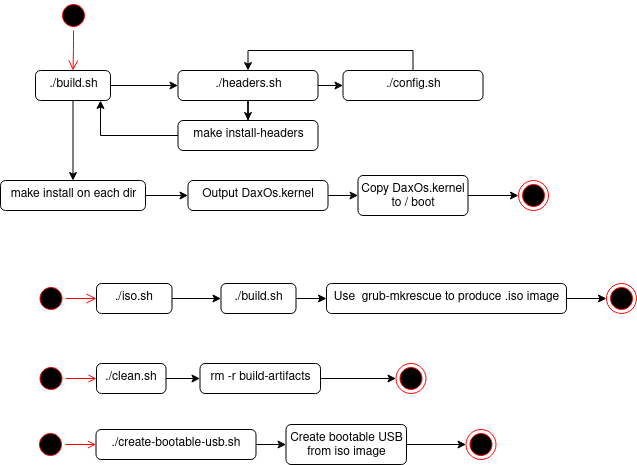
\includegraphics[width=\textwidth,height=\textheight,keepaspectratio]{activity}
	\caption{Activity Diagram}
\end{figure}

\clearpage

\section{Sequence Diagram}

\begin{flushleft}
	This diagram illustrates the time dependent and sequential interaction between the
	user, the OS and the keyboard driver.
	During boot, the Operating System initializes the keyboard driver.
	This involves:
	\begin{enumerate}
		\item \textbf{Self Test}
		\begin{enumerate}
			\item The keyboard device is disabled by sending command 0xAD and 0xA7 to
			the PS/2 controller.
			\item The PS/2 controller's output buffer is flushed by reading from port 0x60.
			\item Initiate the PS/2 controller self test by sending command 0xAA to it. A
			response of 0x55 indicates success.
			\item Enable the keyboard device by sending commands 0xAE and 0xA8 to the
			PS/2 controller.
			\item Reset the device by sending 0xFF to the keyboard.
			\item Set the LED states by sending appropriate commands.
		\end{enumerate}
		\item \textbf{Handling Keypress}
		
		When the user presses a key the keyboard device initiates an interrupt. This done by
		activating IRQ1 which is the standard interrupt line used by keyboards. In response
		to this interrupt, the CPU executes an ISR which updates a buffer with the read
		characters. The I/O functions in stdio.h like scanf will read from this buffer to perform
		the necessary computation and show the results back to the user.
		
	\end{enumerate}
\end{flushleft}

\begin{figure}[h!]
	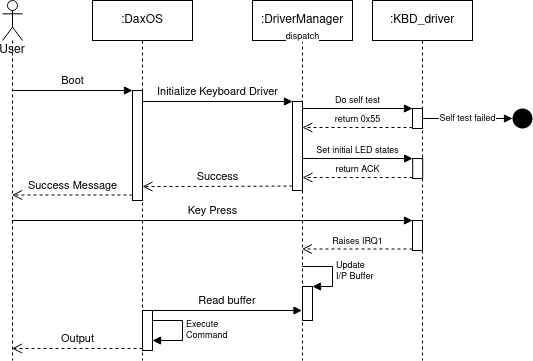
\includegraphics[width=\textwidth,height=\textheight,keepaspectratio]{kbd_driver}
	\caption{Sequence Diagram for keyboard driver}
\end{figure}
\clearpage

\hspace{0pt}
\vfill
\begin{figure}[h!]
	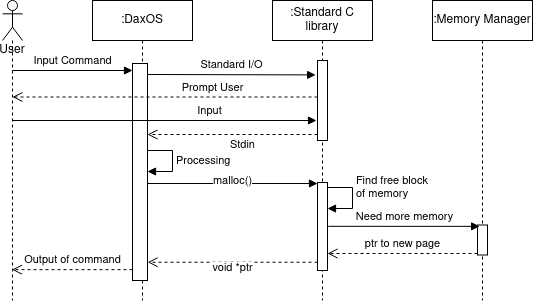
\includegraphics[width=\textwidth,height=\textheight,keepaspectratio]{user_command}
	\caption{Sequence Diagram for user command}
\end{figure}
\hspace{0pt}
\vfill

\pagebreak